\documentclass{standalone}

\usepackage{import}
% 
\usepackage{tikz}
\usepackage{amsmath}
\usetikzlibrary{backgrounds}
% \usepackage{tzplot}

\begin{document}
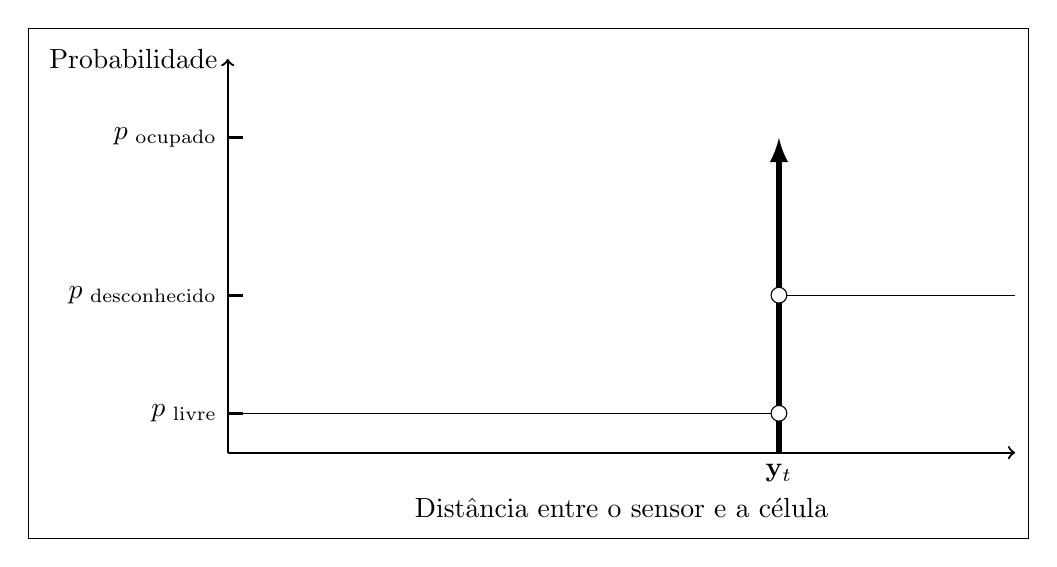
\begin{tikzpicture}[framed]
  \draw[->, thick] (0,0) -- (10,0) node[midway, yshift=-0.7cm] {Distância entre o sensor e a célula};
  \draw[->, thick] (0,0) -- (0,5) node[anchor=east] {Probabilidade};
  \draw[very thick] (0,0.5) node[anchor=east] {$p_\text{ livre}$} -- (0.2, 0.5);
  \draw[](0,0.5)  -- (7,0.5);
  \draw[](7,2) -- (10,2);
  \draw[-latex, line width=2] (7,0) node[anchor=north] {$\mathbf{y}_t$} -- (7, 4.0);
  \draw[fill=white] (7, 0.5) circle (0.1);
  \draw[fill=white] (7, 2) circle (0.1);
  
  \draw[very thick] (0,2) node[anchor=east] {$p_\text{ desconhecido}$} -- (0.2, 2);
  \draw[very thick] (0,4) node[anchor=east] {$p_\text{ ocupado}$} -- (0.2, 4);

\end{tikzpicture}
\end{document}